\chapter{Data and Monte Carlo Simulations}
\label{chapter:MC_simulation}

Monte Carlo (MC) simulation is used to model the signal and Standard Model background processes and to predict their event yields and kinematic distributions.
Event generation begins by sampling the incoming partons and their momentum fractions from proton PDFs and evaluating the matrix element for the hard-scattering process.
The outgoing partons are then evolved through the parton shower and hadronisation, followed by the decays of unstable particles.
Finally, pile-up interactions and the ATLAS detector response are simulated, after which the events are reconstructed with the same algorithms used for collision data.

This chapter describes the collision data and simulation samples used in this thesis.
The Run~2 dataset is presented first, followed by the simulated signal and Standard Model background samples.
The trigger selections are summarised at the end of the chapter.


\section{Dataset selection}
\label{sec:dataset_selection}

The search uses the full LHC Run~2 proton--proton collision dataset recorded by the ATLAS detector between 2015 and 2018 at a centre-of-mass energy of $\sqrt{s}=13~\TeV$.
Only data recorded during stable-beam periods and passing the data-quality requirements are retained~\cite{ATLASDataQualityRun2}.
These periods are defined by the ATLAS good-runs lists (GRLs).

The selected dataset corresponds to an integrated luminosity of $140.1\pm1.2~\ifb$, with a relative uncertainty of $0.83\%$~\cite{ATLASLumiRun2}.
The integrated luminosity recorded in each year is summarised in Table~\ref{tab:run2_luminosity}.

\begin{table}[htbp]
    \centering
    \caption{Integrated luminosity of the Run~2 proton--proton collision data.}
    \label{tab:run2_luminosity}
    \begin{tabular}{cc}
        \hline
        Year & Integrated luminosity [$\ifb$] \\
        \hline
        2015 & $3.24\pm0.04$ \\
        2016 & $33.40\pm0.30$ \\
        2017 & $44.63\pm0.50$ \\
        2018 & $58.79\pm0.64$ \\
        \hline
        Total & $140.07\pm1.17$ \\
        \hline
    \end{tabular}
\end{table}

The mean pile-up during Run~2 was $\langle\mu\rangle\simeq34$, as described in Section~\ref{sec:lhc}.


\section{Signal samples}
\label{sec:signal_samples}

The signal samples implement the $U_{1}$ vector-leptoquark benchmark defined in Section~\ref{subsec:lq_collider_benchmark}. The Yang--Mills scenario with $\kappa_c=\kappa_Y=0$ and $\beta_L^{33}=1$ is used.
The simulated signal covers both the pure-left-handed scenario with $\beta_R^{33}=0$ and the right-handed scenario with $|\beta_R^{33}|=1$.
Apart from their coupling parameters, the same event-generation, parton-shower and detector-simulation settings are used for both scenarios.

\begingroup
\emergencystretch=2em
Signal events are generated at leading order~(LO) in QCD using \textsc{MadGraph5\_\allowbreak aMC@NLO}~3.3.1~\cite{Alwall2014MadGraph}, interfaced to \textsc{Pythia}~8.308~\cite{Bierlich2022Pythia83}.
The hard-scattering process produces a $\tau$-lepton, a $\nu_{\tau}$ and up to two additional partons, which can be gluons or $u$-, $d$-, $s$-, $c$- or $b$-quarks.
The NNPDF3.0nlo PDF set~\cite{Ball2015NNPDF30} is used for the hard-scattering calculation.
\par\endgroup

The generation is performed in the five-flavour scheme, in which the $b$-quark is treated as an active parton in the proton.
The proton PDFs therefore allow processes with an initial-state $b$-quark.
All allowed $U_{1}$ diagrams contributing to this final state are retained in the matrix-element calculation.
The resonant single-production and non-resonant $t$-channel processes shown in Figure~\ref{fig:u1_taunu_target_topologies} are therefore included coherently and cannot be separated at the generation stage.
Other allowed contributions, including leptoquark pair production where kinematically accessible, are also retained.

\textsc{Pythia} subsequently simulates the parton shower and hadronisation.
It also models the underlying event using the A14 tune~\cite{ATLAS2014A14Tune} and the NNPDF2.3lo PDF set~\cite{Ball2013NNPDF23}.
The CKKW--L merging procedure~\cite{Lonnblad2012CKKWL} prevents the same radiation from being included in both the matrix-element and parton-shower calculations.
The Durham $k_{\perp}$ merging scale is set to $15~\GeV$ and the $D$ parameter to 0.4. Together, they determine whether an emission is treated as an additional matrix-element parton or as part of the shower.

For the pure-left-handed interpretation, dedicated signal samples are generated for 152 combinations of $(\MU,\gU,\beta_L^{23})$ satisfying
\begin{align}
    1.5~\TeV &\leq \MU \leq 3.0~\TeV, \\
    0.5 &\leq \gU \leq 3.0, \\
    0 &\leq \beta_L^{23} \leq 2.2,
\end{align}
with $\beta_L^{33}=1$ and $\beta_R^{33}=0$.
The lower boundary of the mass scan covers the region around the exclusion limits obtained from previous leptoquark pair-production searches~\cite{ATLAS2023LQBTau,CMS2021LQThirdGen}.
For $\MU>3~\TeV$, the selected signal is dominated by non-resonant exchange, where the sensitivity is governed mainly by the ratio $\gU/\MU$.
The primary mass scan is therefore restricted to $\MU\leq3~\TeV$.

For the right-handed interpretation with $|\beta_R^{33}|=1$, one baseline sample is generated at each of the six mass points $\MU\in\{1.5,2.0,2.5,3.0,4.0,5.0\}~\TeV$ with $\gU=1$ and $\beta_L^{23}=0.2$.
Predictions at other values of $\gU$ and $\beta_L^{23}$ are obtained from these baseline samples using corrected \textsc{MadGraph5\_aMC@NLO} internal event weights, rather than from separately generated samples at every parameter point.
The correction includes an adjustment of the normalisation and a two-dimensional truth-level shape correction based on the leading-jet $\pT$ and $m_{b\tau}$.
Details of the correction and its validation are given in Appendix~\ref{app:signal_weight_correction}.
This strategy avoids repeating event generation and detector simulation for every coupling configuration, thereby reducing the required computing resources.

The $U_{1}$ amplitude can interfere with the SM amplitude for production of the same $\tau\nu_{\tau}+\mathrm{jets}$ final state.
The total matrix element can be expressed as
\begin{align}
    \left|\mathcal{M}_{\mathrm{SM}}+\mathcal{M}_{U_1}\right|^{2}
    =
    \left|\mathcal{M}_{\mathrm{SM}}\right|^{2}
    +
    \left|\mathcal{M}_{U_1}\right|^{2}
    +
    2\,\mathrm{Re}
    \left(
        \mathcal{M}_{\mathrm{SM}}
        \mathcal{M}_{U_1}^{*}
    \right).
    \label{eq:signal_interference}
\end{align}
The first term represents the SM contribution, the second represents the pure $U_{1}$ contribution, corresponding to the BSM-only component, and the third represents their interference.
Unlike the BSM-only component, the interference term can be negative and can reduce the predicted yield relative to the SM-only expectation in some regions of phase space.

To separate the BSM-only and interference terms in Eq.~\eqref{eq:signal_interference}, the two contributions are generated independently.
The BSM-only component is selected by requiring exactly two new-physics couplings at the amplitude level, denoted by \texttt{NP==2}, whereas the interference component is isolated at the squared-matrix-element level by requiring \texttt{NP\^{}2==2}.
The interference sample therefore contains only the third term in Eq.~\eqref{eq:signal_interference}.

All $\tau$-lepton decay modes are retained in the signal simulation.
Although the signal regions target hadronically decaying $\tau$-leptons, leptonic decays can contribute to regions containing electrons or muons.
The inclusive decay configuration allows this signal contamination to be evaluated.

The decays of bottom- and charm-hadrons are simulated with \textsc{EvtGen}~\cite{Lange2001EvtGen}.
All signal samples used in this thesis are processed with the ATLAS fast detector simulation \textsc{AtlFast3}~\cite{ATLAS2022AtlFast3}, which provides a computationally efficient simulation of the calorimeter response.

\section{Background samples}
\label{sec:background_samples}

The simulated SM backgrounds considered in this analysis are $\wjets$, $\zjets$, $\ttbar$, single-top and diboson production.
The dominant contribution is $\wtaunu+\mathrm{jets}$ production.
The QCD multijet background is negligible after event cleaning and is therefore neglected, as discussed in Section~\ref{subsec:ch7_multijet} and Appendix~\ref{App:QCD_bkg_study}.

The $\wzjets$ samples are generated with \textsc{Sherpa}~2.2.11~\cite{Bothmann2019Sherpa22}, except for $\ztautau$, which uses version~2.2.14.
Matrix elements include up to two additional partons at next-to-leading order~(NLO) in QCD and up to five at LO.
They are merged with the \textsc{Sherpa} parton shower~\cite{Schumann2008SherpaPS} using the MEPS@NLO prescription~\cite{Hoche2012MEPSNLO,Hoche2013MEPSNLO,Catani2001MEPS,Hoche2009MEPS}.

Only a small fraction of inclusive $\wtaunu$ events passes the high-$\met$ requirement, leaving limited MC statistics.
Two dedicated filtered samples are therefore used to reduce the MC statistical uncertainty in the high-$\met$ tail.
Their respective generator-level requirements are
\begin{align}
    70~\GeV < \met < 150~\GeV
    &\quad\mathrm{and}\quad
    \pT^{\tau} < 150~\GeV, \notag\\
    \met > 150~\GeV
    &\quad\mathrm{or}\quad
    \pT^{\tau} > 150~\GeV.
\end{align}

Top-quark pair and single-top production are generated at NLO accuracy in QCD using \textsc{Powheg Box}~v2~\cite{Frixione2007PowhegHF,Nason2004Powheg,Frixione2007Powheg,Alioli2010PowhegBox}, interfaced to \textsc{Pythia}~8.230~\cite{Sjostrand2015Pythia82} for parton showering and hadronisation.
The single-top samples include $s$-channel, $t$-channel and $Wt$ production. 
The predicted $\ttbar$ yield is normalised to the inclusive production cross-section calculated at next-to-next-to-leading order~(NNLO) in QCD with next-to-next-to-leading-logarithmic~(NNLL) soft-gluon resummation~\cite{CzakonMitov2014TopPP}.
A dilepton filter is applied to the $\ttbar$ sample, requiring both $W$ bosons to decay leptonically.
Diboson production is modelled with \textsc{Sherpa}~2.2.11 and~2.2.12.

The hard-scattering calculations use the NNPDF3.0nnlo PDF set for $\wzjets$ and NNPDF3.0nlo for $\ttbar$ and single-top production~\cite{Ball2015NNPDF30}.
The underlying event is modelled using the A14 tune for \textsc{Pythia} and the default tune for \textsc{Sherpa}.
For samples not generated with \textsc{Sherpa}, the decays of bottom- and charm-hadrons are modelled with \textsc{EvtGen}~\cite{Lange2001EvtGen}.
The full ATLAS detector simulation based on \textsc{Geant4}~\cite{ATLAS2010Simulation,Agostinelli2003Geant4} is used for all background samples.
The MC generator configurations are summarised in Table~\ref{tab:mc_generator_summary}.

\begin{table}[htbp]
    \centering
    \caption{
        Summary of the MC generator configurations used for the signal and SM background processes.
    }
    \label{tab:mc_generator_summary}
    \resizebox{\textwidth}{!}{
    \begin{tabular}{llllll}
        \toprule
        Process
        & Generator
        & ME order
        & Parton shower
        & PDF set
        & Tune \\
        \midrule

        $U_{1}$ signal
        & \textsc{MadGraph5\_aMC@NLO} 3.3.1
        & LO
        & \textsc{Pythia} 8
        & NNPDF3.0nlo
        & A14 \\
        \midrule

        $W(\rightarrow e\nu/\mu\nu/\tau\nu)+\mathrm{jets}$
        & \textsc{Sherpa} 2.2.11
        & NLO
        & \textsc{Sherpa}
        & NNPDF3.0nnlo
        & \textsc{Sherpa} \\

        $Z(\rightarrow ee/\mu\mu/\nu\nu)+\mathrm{jets}$
        & \textsc{Sherpa} 2.2.11
        & NLO
        & \textsc{Sherpa}
        & NNPDF3.0nnlo
        & \textsc{Sherpa} \\

        $Z(\rightarrow \tau\tau)+\mathrm{jets}$
        & \textsc{Sherpa} 2.2.14
        & NLO
        & \textsc{Sherpa}
        & NNPDF3.0nnlo
        & \textsc{Sherpa} \\

        $\ttbar$
        & \textsc{Powheg Box} v2
        & NLO
        & \textsc{Pythia} 8
        & NNPDF3.0nlo
        & A14 \\

        Single-$t$
        & \textsc{Powheg Box} v2
        & NLO
        & \textsc{Pythia} 8
        & NNPDF3.0nlo
        & A14 \\

        Diboson
        & \textsc{Sherpa} 2.2.11/2.2.12
        & NLO/LO
        & \textsc{Sherpa}
        & NNPDF3.0nnlo
        & \textsc{Sherpa} \\

        \bottomrule
    \end{tabular}
    }
\end{table}

\section{Triggers}
\label{sec:analysis_triggers}

The ATLAS Run~2 trigger architecture was described in Chapter~\ref{chapter:LHC_ATLAS_experiment}.
Single-electron, single-muon and $\met$ triggers are used in this analysis.

The signal region event selection uses the lowest-threshold unprescaled $\met$ trigger, which is fully efficient for the offline requirement $\met>200~\GeV$ applied in the signal regions and the corresponding validation regions.
Single-electron and single-muon triggers are used in regions containing an electron or muon.
The lowest online thresholds range from $20$ to $26~\GeV$~\cite{ATLASElectronTriggerRun2,ATLASMuonTriggerRun2}.

Table~\ref{tab:run2_trigger_chains} lists the trigger chains used in this analysis.
In an HLT chain name, \texttt{e}, \texttt{mu} and \texttt{xe} represent an electron, a muon and $\met$, respectively. The following number gives the online threshold in \GeV.
The \texttt{L1} suffix indicates the first-level trigger that seeds the chain.
The electron labels \texttt{lhloose}, \texttt{lhmedium} and \texttt{lhtight} specify likelihood-based identification requirements, while \texttt{nod0} indicates that transverse-impact-parameter information is omitted.
The labels \texttt{iloose}, \texttt{ivarloose} and \texttt{ivarmedium} specify isolation requirements.
For $\met$, \texttt{mht} denotes a calculation based on the negative vector sum of jet transverse momenta, whereas \texttt{pufit} denotes a calorimeter-based calculation with a fit-based pile-up correction~\cite{ATLASMETTriggerRun2}.

Figures~\ref{fig:run2_lepton_trigger_efficiency} and~\ref{fig:run2_met_trigger_efficiency} show representative Run~2 trigger-efficiency measurements.
Differences in trigger efficiency between collision data and simulation are corrected using data-to-simulation efficiency scale factors.


% Source: TauX_Gnt1makerAlg/python/TriggerList.py, Obsidian snapshot 2026-09-08.
% Run-2 entries of trig_singleEle, trig_singleMuon and trig_met.
% Single-lepton OR and MET period selection checked in
% TauXFastFrame/Root/TauXHelpers.cc: getSLTflag and getMETflag.
\begin{table}[htbp]
    \centering
    \caption[Run~2 single-lepton and missing-transverse-momentum trigger chains]{
        Single-electron, single-muon and $\met$ trigger chains used in the Run~2 analysis.
        Single-lepton chains listed for the same flavour and year are combined with a logical OR, while the $\met$ chain is selected according to the data-taking period.
    }
    \label{tab:run2_trigger_chains}
    \begingroup
    \small
    \setlength{\tabcolsep}{4pt}
    \renewcommand{\arraystretch}{1.08}
    \begin{tabular}{lll}
        \toprule
        Trigger & Year & HLT chain \\
        \midrule
        Single-electron & 2015 & \texttt{\detokenize{HLT_e24_lhmedium_L1EM20VH}} \\
        & & \texttt{\detokenize{HLT_e60_lhmedium}} \\
        & & \texttt{\detokenize{HLT_e120_lhloose}} \\
        & 2016--2018 & \texttt{\detokenize{HLT_e26_lhtight_nod0_ivarloose}} \\
        & & \texttt{\detokenize{HLT_e60_lhmedium_nod0}} \\
        & & \texttt{\detokenize{HLT_e140_lhloose_nod0}} \\
        \midrule
        Single-muon & 2015 & \texttt{\detokenize{HLT_mu20_iloose_L1MU15}} \\
        & & \texttt{\detokenize{HLT_mu40}} \\
        & 2016--2018 & \texttt{\detokenize{HLT_mu26_ivarmedium}} \\
        & & \texttt{\detokenize{HLT_mu50}} \\
        \midrule
        $\met$ & 2015 & \texttt{\detokenize{HLT_xe70_mht}} \\
        & 2016 & \texttt{\detokenize{HLT_xe90_mht_L1XE50}} \\
        & & \texttt{\detokenize{HLT_xe100_mht_L1XE50}} \\
        & & \texttt{\detokenize{HLT_xe110_mht_L1XE50}} \\
        & 2017 & \texttt{\detokenize{HLT_xe110_pufit_L1XE55}} \\
        & & \texttt{\detokenize{HLT_xe110_pufit_L1XE50}} \\
        & 2018 & \texttt{\detokenize{HLT_xe110_pufit_xe70_L1XE50}} \\
        & & \texttt{\detokenize{HLT_xe110_pufit_xe65_L1XE50}} \\
        \bottomrule
    \end{tabular}
    \endgroup
\end{table}

\begin{figure}[htbp]
    \centering
    \begin{subfigure}{0.62\textwidth}
        \centering
        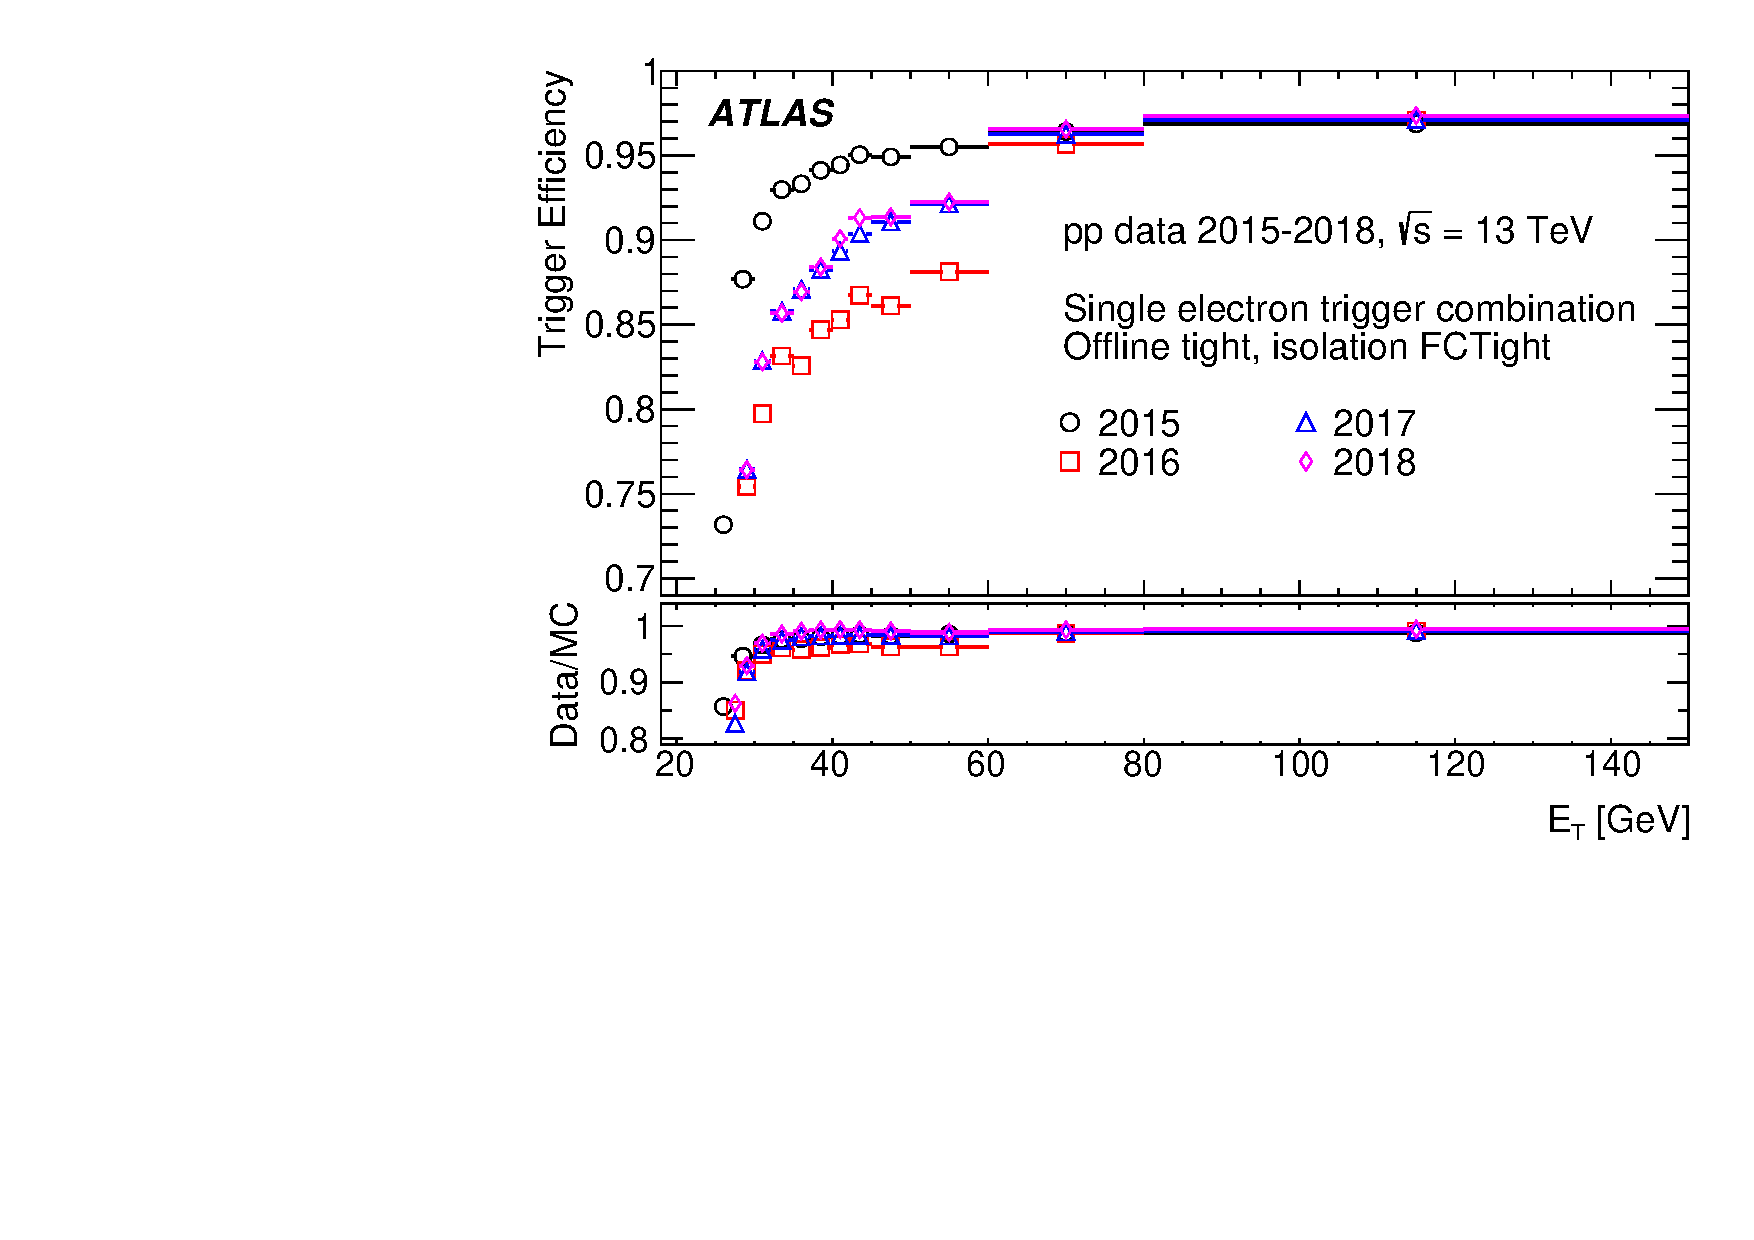
\includegraphics[width=\linewidth]{Figs/CH5/trigger_electron_efficiency.pdf}
        \caption{Single-electron trigger combination.}
    \end{subfigure}
    \par\medskip
    \begin{subfigure}{0.48\textwidth}
        \centering
        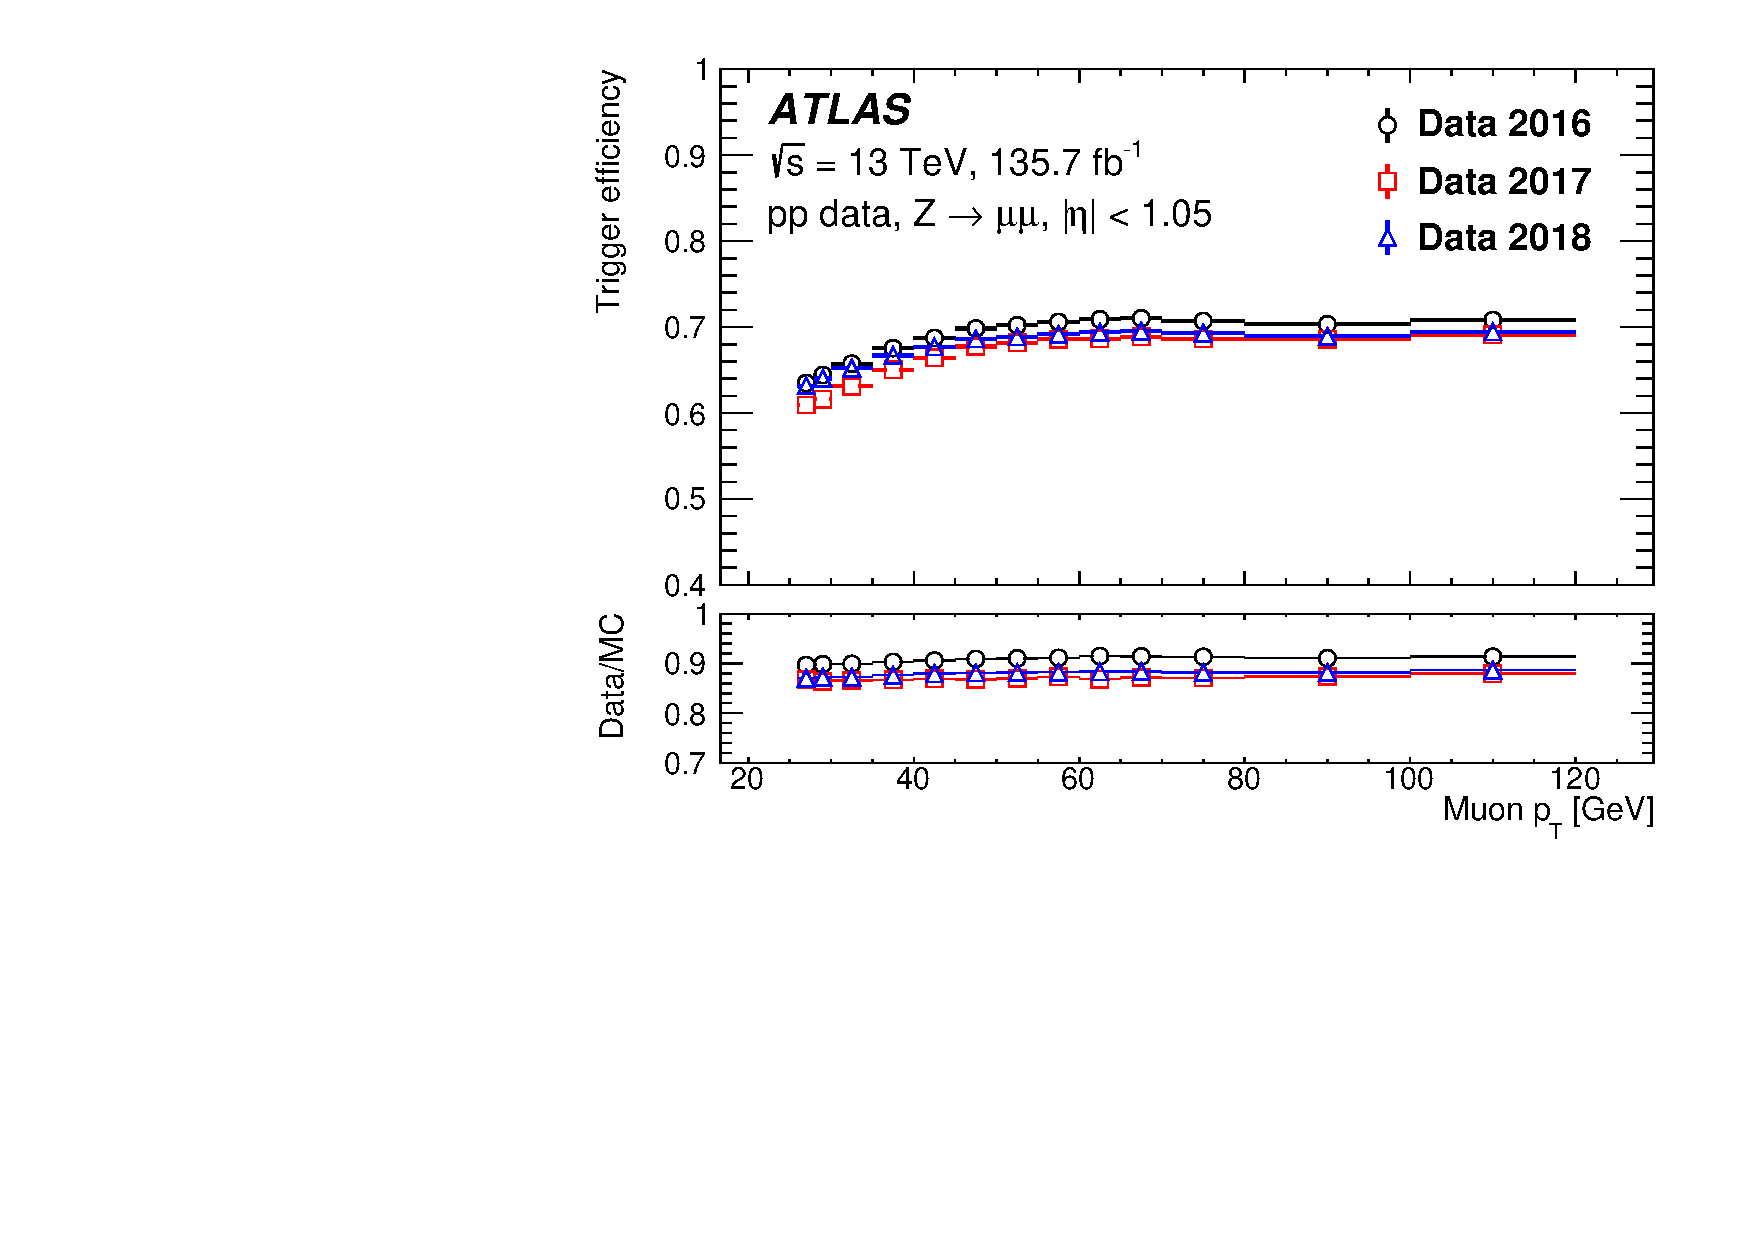
\includegraphics[width=\linewidth]{Figs/CH5/trigger_muon_efficiency_barrel.pdf}
        \caption{Single-muon triggers, barrel.}
    \end{subfigure}
    \hfill
    \begin{subfigure}{0.48\textwidth}
        \centering
        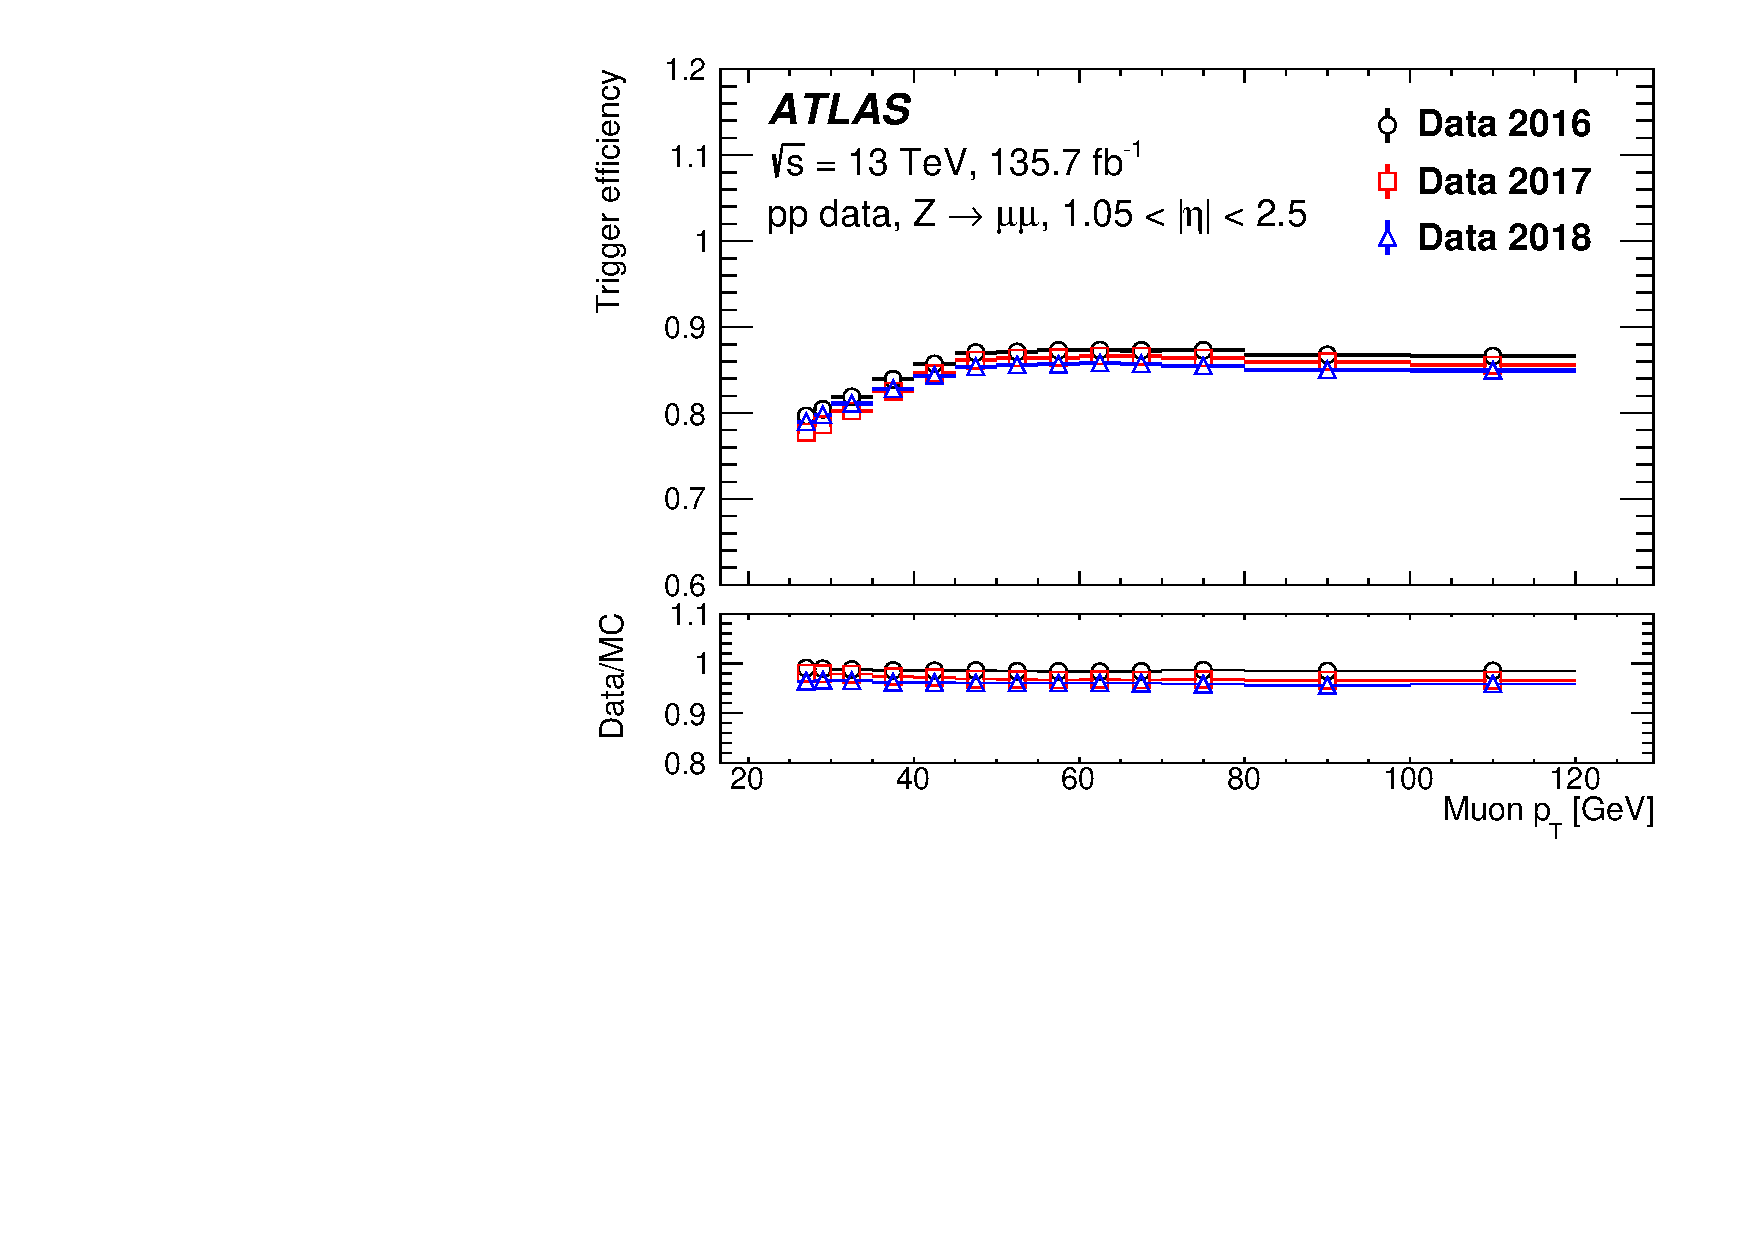
\includegraphics[width=\linewidth]{Figs/CH5/trigger_muon_efficiency_endcap.pdf}
        \caption{Single-muon triggers, end-cap.}
    \end{subfigure}
    \caption[Run~2 single-lepton trigger efficiencies]{
        Single-lepton trigger efficiencies measured in Run~2 $\zll$ events.
        (a) Electron efficiency versus offline $\et$ for electrons with Tight identification and FCTight isolation~\cite{ATLASElectronTriggerRun2}.
        (b,c) Muon efficiency versus offline $\pT$ in the barrel and end-cap regions, respectively~\cite{ATLASMuonTriggerRun2}.
        Electron uncertainties include statistical and systematic contributions, while muon uncertainties are statistical only.
    }
    \label{fig:run2_lepton_trigger_efficiency}
\end{figure}

\begin{figure}[htbp]
    \centering
    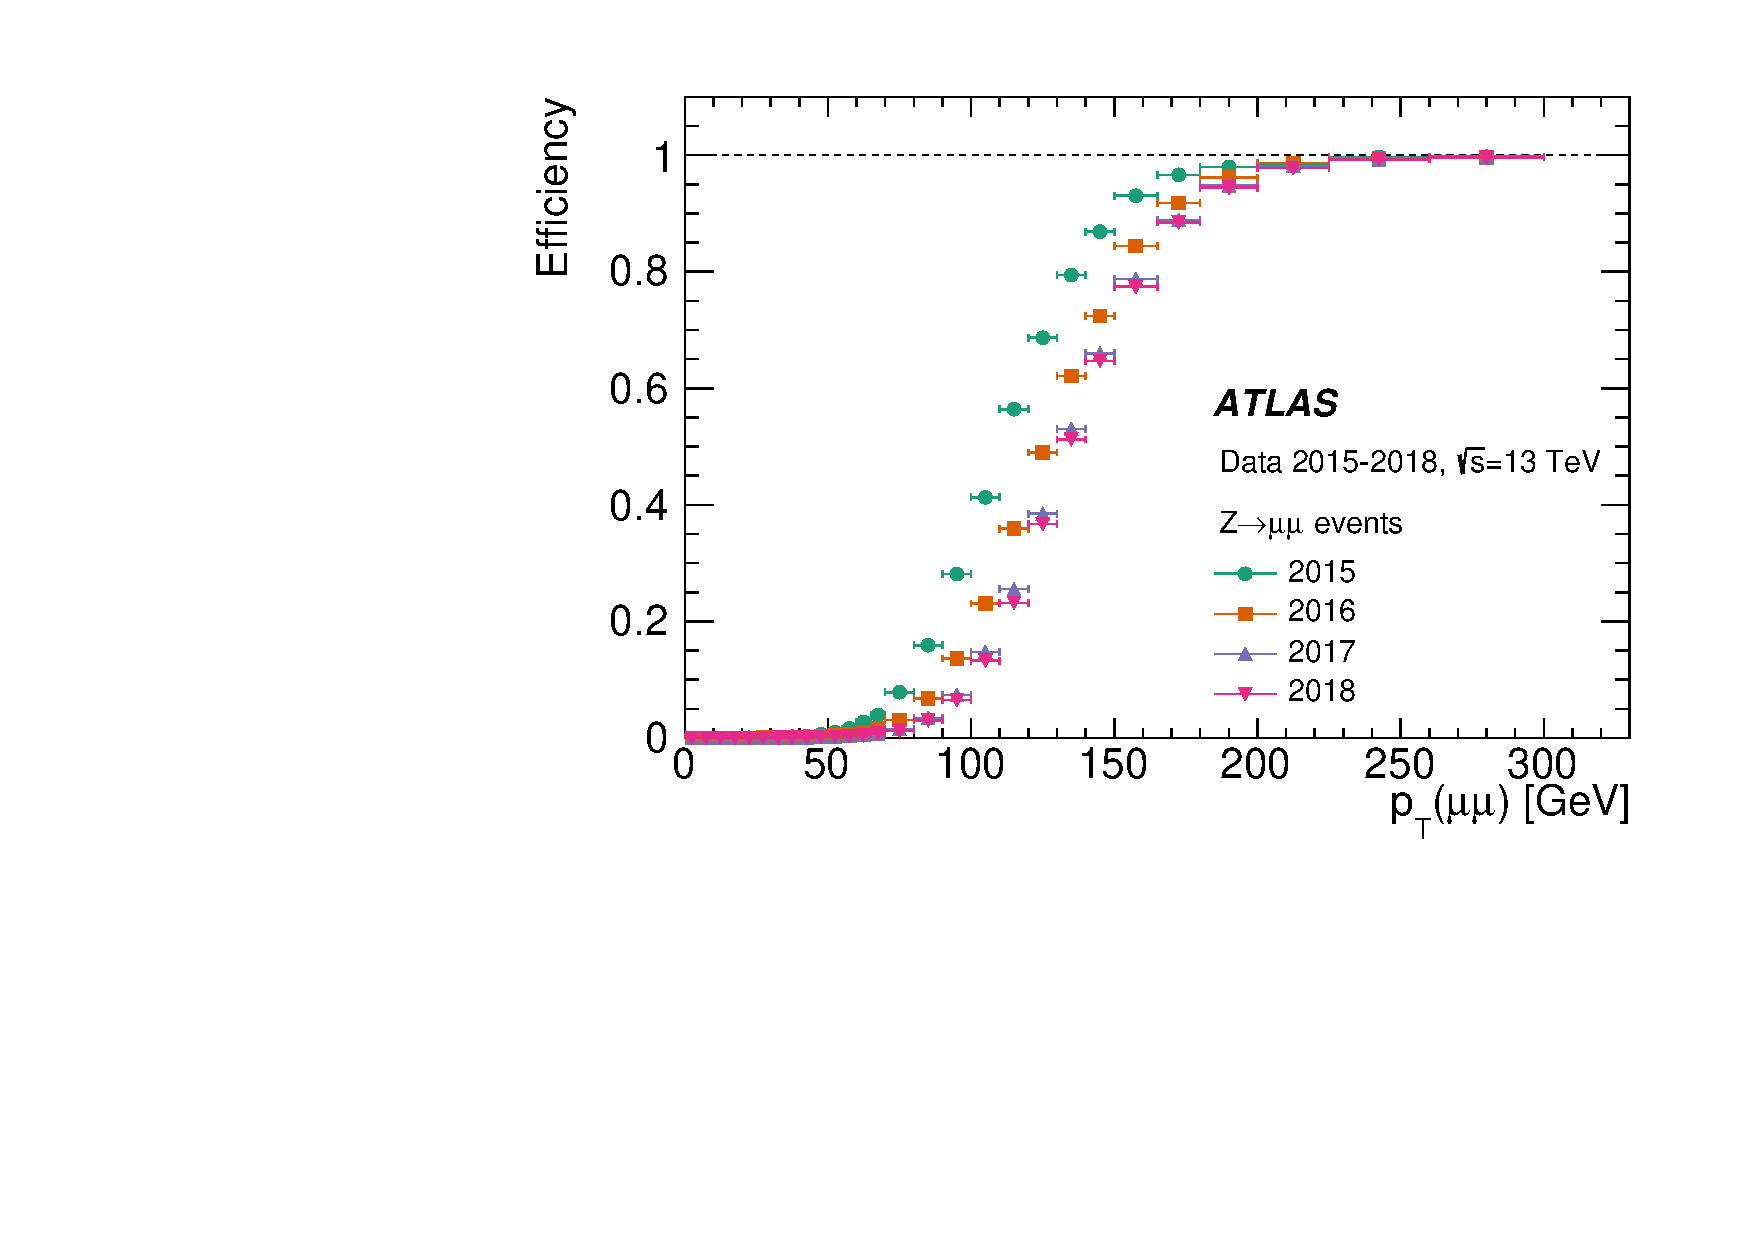
\includegraphics[width=0.72\textwidth]{Figs/CH5/trigger_met_efficiency.pdf}
    \caption[Run~2 missing-transverse-momentum trigger efficiencies]{
        Combined L1 and HLT $\met$ trigger efficiencies in $\zmumu$ events for each year of Run~2~\cite{ATLASMETTriggerRun2}.
        Since muons are treated as invisible by these calorimeter-based triggers, the dimuon transverse momentum $\pT(\mu\mu)$ provides a reference for the missing transverse momentum measured by the trigger.
        The curves use the lowest unprescaled trigger as it changes within each year. Error bars show statistical uncertainties.
    }
    \label{fig:run2_met_trigger_efficiency}
\end{figure}
